% Generated by tex/build_swebok_structure.py from tex/chapters/ch01/03_ソフトウェア要求の基礎.tex
\subsubsection{なぜこのように要求を分類するのか}

要求を分類する理由は、実務上は非常に明確である。

\begin{itemize}
\item 要求の種類によって、要求の源泉が異なる。
\item 源泉が異なれば、聞き出し方も異なる。
\item 種類によって、分析方法、仕様化方法、確認すべき相手が異なる。
\item 要求の種類によって、設計・実装・テストへの影響が異なる。
\end{itemize}

さらに、分類は複雑さを下げる。業務規則を議論している最中に、同時にデータベース製品や処理速度を議論すると、論点が混ざる。機能要求、技術制約、サービス品質制約を分ければ、業務の専門家は業務の観点に集中でき、技術者は技術の観点に集中できる。

\MiniBox{完全技術フィルタ}{機能要求と非機能要求の境界が曖昧なときは、「無限に速く、記憶容量が無限で、費用がゼロで、故障しない理想的なコンピュータがあっても、その要求を書く必要があるか」と問う。必要なら機能要求である。不要なら、技術や品質に関する制約、つまり非機能要求である。}

\begin{figure}[htbp]
\centering
\IfFileExists{swebok_structure/CH01.ソフトウェア要求(Software_Requirements)/1.1.ソフトウェア要求の基礎(Software_Requirements_Fundamentals)/1.1.8.なぜこのように要求を分類するのか(Why_Categorize_Requirements_This_Way)/assets/fig-ch01-03.png}{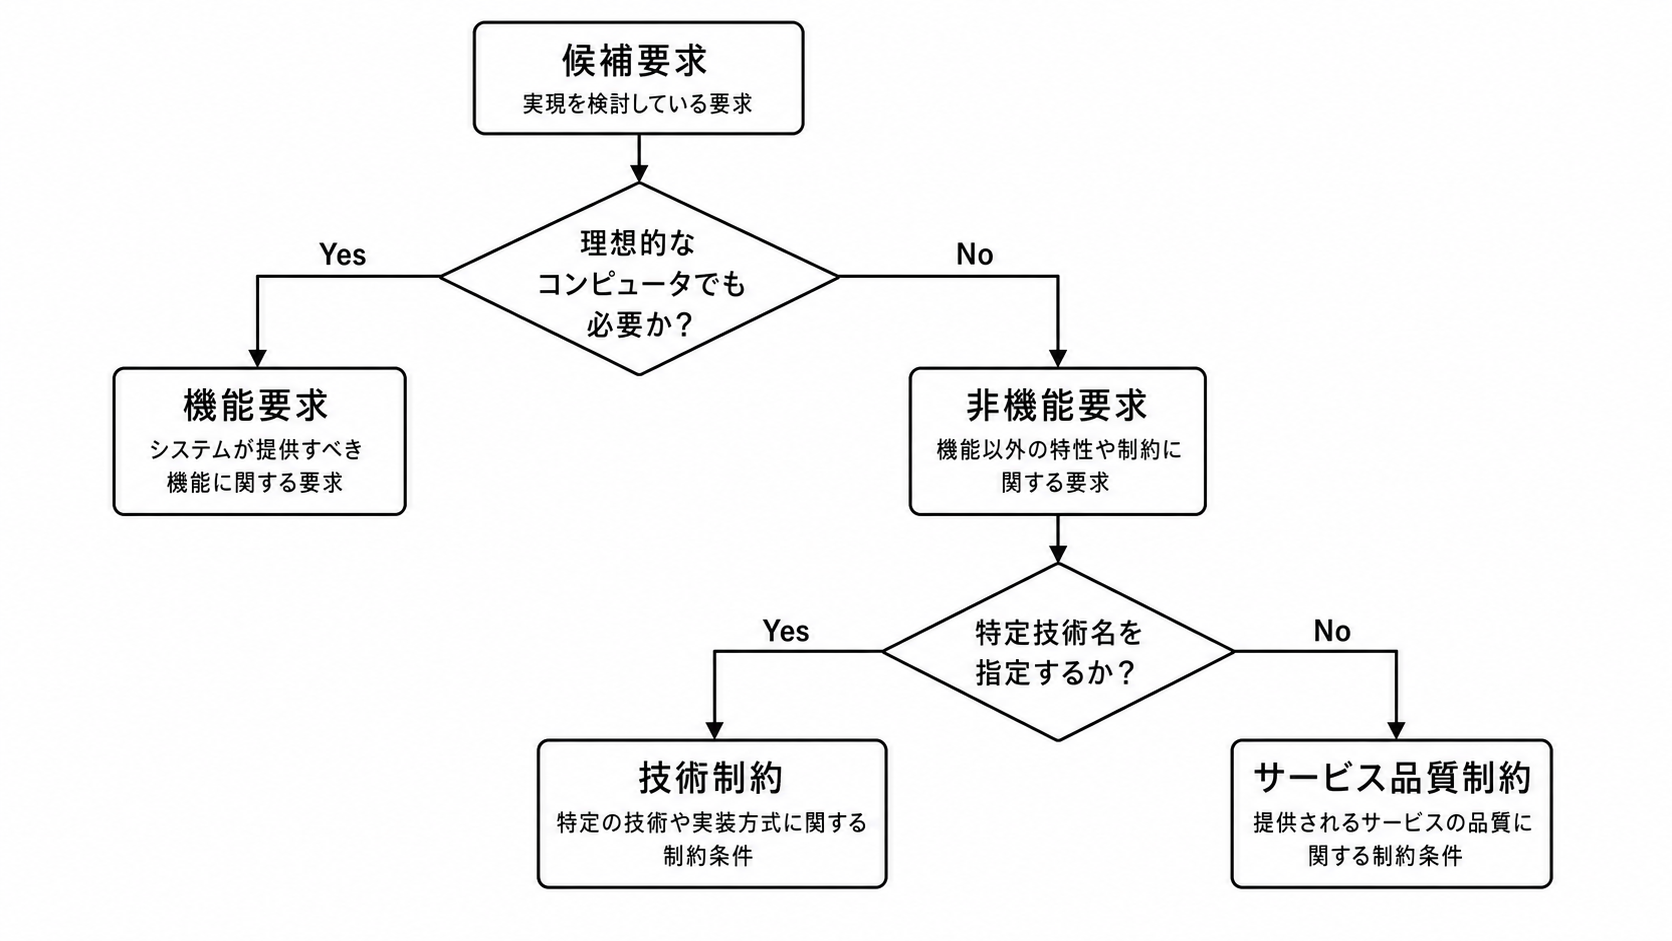
\includegraphics[width=0.96\linewidth]{swebok_structure/CH01.ソフトウェア要求(Software_Requirements)/1.1.ソフトウェア要求の基礎(Software_Requirements_Fundamentals)/1.1.8.なぜこのように要求を分類するのか(Why_Categorize_Requirements_This_Way)/assets/fig-ch01-03.png}}{\fbox{\parbox[c][48mm][c]{0.9\linewidth}{\centering 画像生成待ち\\完全技術フィルタの判定フロー}}}
\caption{完全技術フィルタの判定フロー}
\label{fig:ch01-03}
\end{figure}
